\textbf{Ziele:}\\
Entwicklungszeit $\downarrow$, Fehler $\downarrow$, Fertigungsverfahren planen, 
Fertigung optimieren, Ausschuss $\downarrow $, Zusammenhänge 
verstehen und vorhersehen, Kosten planen\\

\textbf{Typen:}
\begin{itemize}
    \item Analytische/nichtumerische Simulation (CFD, FEM)
    \item Grafische Simulation (CAD, VR)
    \item Realexperimente
\end{itemize}
\hspace{0.05\linewidth}

\textbf{Möglichkeiten:}\\
Giessprozesse (Formfüllung Erstarrung), Umformen (Kraft, Spannungen, Mikrostruktur), Zerspanung (Spanbildung, Thermik), Fügen (Schweissnähte, Verzug, Einflusszone), Werkstoffe (mikrostruktur, Gefüge, Kristalle) \\

\textbf{Schritte zur FE Lösung:}\\
Zu lösendes Problem $\rightarrow$ Variationsformulierung $\rightarrow$ Diskretisierung $\rightarrow$ Assemblierung\\ $\rightarrow$ Lösung der DGL\\
%\vfill \null \columnbreak

\textbf{Wahre vs FEM Lösung:}\\
Im FEM wird nur an endlich vielen Punkten gerechnet. Mit der FEM-Lösung wird die ursprüngliche DGL nicht notwendigerweise exakt erfüllt. \\

\textbf{Fehlerquellen:} 
Phsikalisches System, Mathematisches Modell, Diskretes Modell, FEM Lösung \\

Die \textbf{Analytische} Lösung erfüllt Feldproblem auf gesamten Lösungsgebiet.

Für \textbf{FEM bei thermischen Problemen} werden drei unabhängige Kennwerte (Wärmekapazität $c$, Wärmeleitfähigkeit $\lambda$, Dichte $\rho$) benötigt.\\

\textbf{1D Wärmeleitung mit FEM:} $\frac{\partial T}{\partial t} = - \frac{k}{c_p \rho }\Delta T$

\subsection*{Nichtlinearitäten:}
bei \textbf{grossen Deformationen}, \textbf{Reibung} und \textbf{Zeitabhängigkeit}\\
Die Lösung ist dann nicht in einem Schritt möglich, sondern via Iteration (Zeitdiskretisierung).\\ 

Es gibt drei Arten von Nichtlinearitäten:
\begin{itemize}
    \item Geometrisch: Verformung zu gross
    \item Materialbasiert: nichtlineares Materialverhalten
    \item Strukturbasiert: Lagerbedingungen verändern sich
\end{itemize}
Bei Zerspanung treten alle drei auf.

\subsection{Implizite vs. explizite FEM}

\textbf{Implizit:} \\
\begin{minipage}{0.45\linewidth}
    \begin{plusitemize}
        \item Grössere Zeitschritte möglich 
        \item stabiles Verfahren falls Konvergenz
        \item Effektiv bei kleinen, linearen und statischen Problemen
    \end{plusitemize}
\end{minipage}
\begin{minipage}{0.5\linewidth}
    \begin{minusitemize}
        \item Hoher Zeitaufwand 
        \item Keine Konvergenz bei Instabilitäten (Beulen oder Falten)
    \end{minusitemize}
\end{minipage}
\\

\textbf{Explizit:} \\
\begin{minipage}{0.45\linewidth}
    \begin{plusitemize}
        \item Gut für hochdynamische, grosse Systeme
        \item Gut bei Nichtlinearitäten
        \item Sehr effektiv bei diagonaler Massematrix 
        \item schnellere Konvergenz
    \end{plusitemize}
\end{minipage}
\begin{minipage}{0.5\linewidth}
    \begin{minusitemize}
        \item kleinere Zeitschritte
        \item Bedingt stabil
        \item Skalierung von Masse oder Zeit führt zu dynamischen Effekten
        \item numerische Fehler schwer abschätzbar
    \end{minusitemize}
\end{minipage}
\begin{center}
    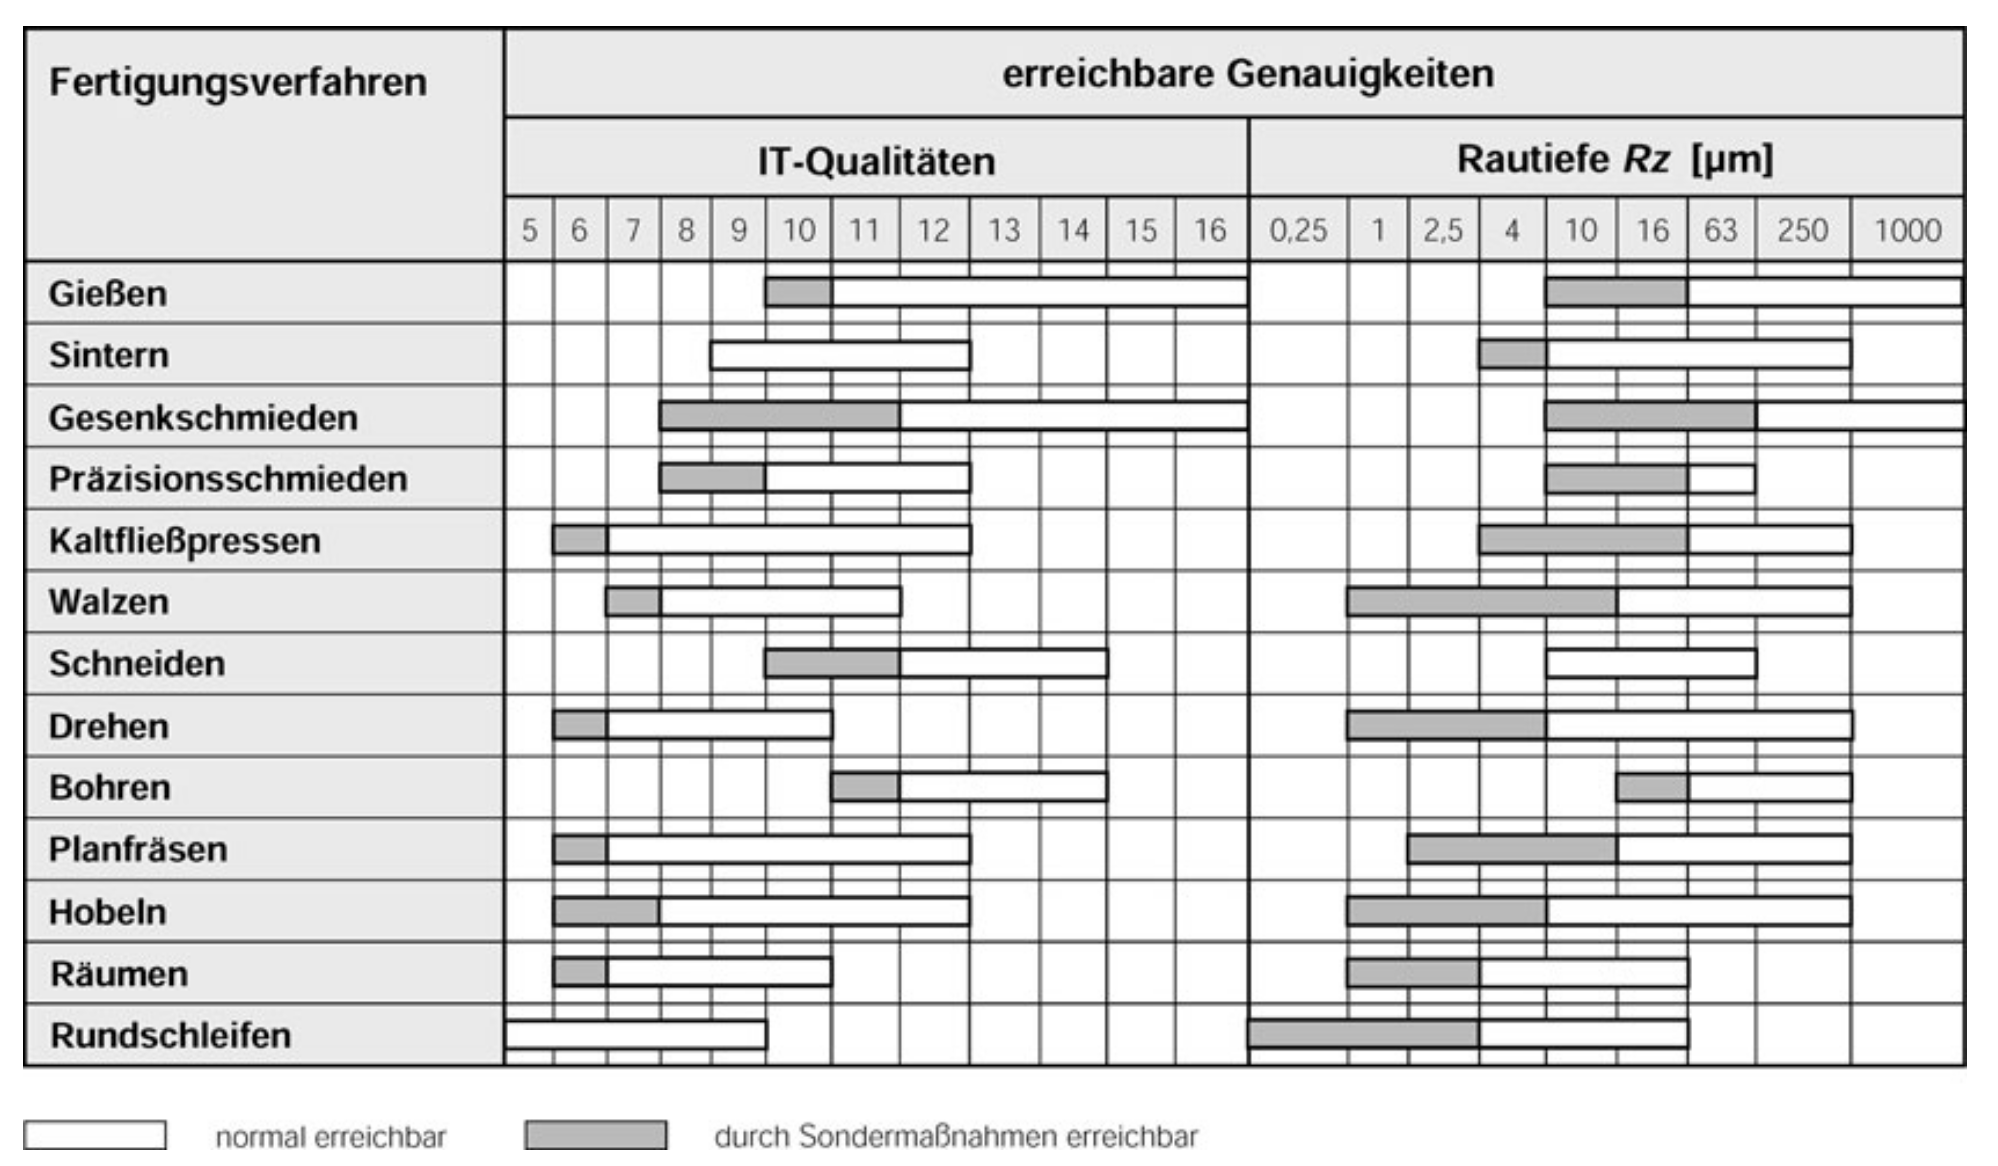
\includegraphics[width=0.9\linewidth]{src/images/Genauigkeiten.png}
\end{center}
